\documentclass{article}

\usepackage[utf8]{inputenc}
\usepackage[brazilian]{babel}
\usepackage{graphicx}
\usepackage{float}
\usepackage[pdftex]{hyperref}
\usepackage{epstopdf}
\usepackage{etoolbox}
\usepackage{amsmath}
\usepackage{amsfonts}
\usepackage{amssymb}
\usepackage{caption}
\usepackage{subcaption}
\usepackage{setspace}
\usepackage{tikz}

\patchcmd{\thebibliography}{\section*}{\section}{}{}
\newcommand{\R}{\ensuremath{\mathbb{R}}}
\newcommand{\Prob}{\ensuremath{\mathbb{P}}}
\newcommand{\K}{\ensuremath{\mathbb{K}}}
\newcommand{\U}{\ensuremath{\mathbb{U}}}
\newcommand{\N}{\ensuremath{\mathbb{N}}}
\newcommand{\Lg}{\ensuremath{\mathbb{L}}}
\newcommand{\T}{\ensuremath{\rm Tr}}
\newcommand{\sg}{{\sigma(x_k)}}

\newcommand{\G}{\ensuremath{\mathcal{G}}}
\newcommand{\F}{\ensuremath{\mathcal{F}}}
\newcommand{\C}{\ensuremath{\mathcal{C}}}
\newcommand{\E}{\ensuremath{\mathcal{E}}}
\newcommand{\Hn}{\ensuremath{\mathcal{H}}}
%\newcommand{\Hoo}{\ensuremath{\mathcal{H}_\infty}}
\newcommand{\Hop}{\ensuremath{\mathcal{H}_{op}}}
% --------------------------------------------------
\newtheorem{theo}{Teorema}
\newtheorem{exa}{Exemplo}
\newtheorem{lemm}{Lema}
\newtheorem{coro}{Corolário}
\newtheorem{defn}{Definição}[section]

%opening


\begin{document}

\begin{titlepage}
\begin{center}

\newcommand{\HRule}{\rule{\linewidth}{0.5mm}}
% Upper part of the page. The '~' is needed because \\
% only works if a paragraph has started.

\includegraphics[width=0.15\textwidth]{logoUnicamp}~\\[1cm]

\textsc{\LARGE Universidade Estadual de Campinas}\\[1.5cm]

\textsc{\Large Faculdade de Engenharia Mecânica}\\[0.5cm]

% Title
\HRule \\[0.4cm]
{ \huge \bfseries ES827 - Robótica Industrial\\ \vspace{1cm} Projeto Final \\
\Large{Dinâmica e Cinemática do Robô Puma 560} \\[0.4cm] }

\HRule \\[1.5cm]

% Author and supervisor
\begin{minipage}{0.6\textwidth}
\begin{flushleft} \large
\emph{Nome:}\\
Daniel Dello Russo Oliveira\\ Marcelli Tiemi Kian
\end{flushleft}
\end{minipage}
\begin{minipage}{0.2\textwidth}
\begin{flushright} \large
\emph{RA}\\ 101918\\
117892
\end{flushright}
\end{minipage}

\vfill

% Bottom of the page
{\large \today}

\end{center}
\end{titlepage}


\onehalfspacing
\section{Objetivos} 
O objetivo desse projeto é simular e analisar aspectos dinâmicos de um robô Puma 560, e cinemática de um robô criado pelo arquivo ``ini\_Rbt.m"\cite{bb:inirbt} conforme sugerido pelo roteiro\cite{bb:roteiro}.
	
\section{Dinâmica do Puma 560}
Pelo roteiro foi sugerido para a análise dinâmica, utilizar o robô Puma 560 construído automaticamente pela ``toolbox" de robótica\cite{bb:toolbox}, a função ``accel" e a ``Matlab Function" pelo Simulink. Entretanto, algumas modificações foram feitas. Retiramos o atrito seco (de Coulomb) nas juntas do robô, pois gerava longos tempos de simulação, e utilizamos um ``script" do Matlab em vez de usar o Simulink.

\subsection{Malha aberta}
A seção 6.3 da tese\cite{bb:tese} utilizada como base mostra simulações feitas com o robô em malha aberta. A partir de entradas desejadas para $q_{des}$ e $\dot{q_{des}}$ calculamos o vetor de torque $u$ necessário para manter a posição. Como podemos observar, fizemos as simulações abaixo utilizando o robô Puma 560 também em malha aberta para as mesmas condições iniciais informadas pela tese\cite{bb:tese}, mas com o vetor $u$ calculado para o robô Puma 560.

\begin{equation}
\label{eq:qdesejado}
q_{des}=\begin{bmatrix}
0 & \frac{\pi}{2} & -\frac{\pi}{2} & 0 & 0 & 0
\end{bmatrix}^T
\end{equation}

\begin{equation}
\label{eq:qddesejado}
\dot{q_{des}}=\begin{bmatrix}
0 & 0 & 0 & 0 & 0 & 0
\end{bmatrix}^T
\end{equation}

\begin{equation}
\label{eq:torques}
u=\begin{bmatrix}
0 & 0 & 0 & 0 & 0 & 0 %TODO: escrever vetor de torques
\end{bmatrix}^T
\end{equation}

\subsubsection{Simulação 1}
Condições iniciais:
\begin{equation}
\label{eq:sim1q}
q_{init}=\begin{bmatrix}
0 & 0 & 0 & 0 & 0 & 0
\end{bmatrix}^T
\end{equation}
\begin{equation}
\label{eq:sim1qd}
\dot{q_{init}}=\begin{bmatrix}
0 & 0 & 0 & 0 & 0 & 0
\end{bmatrix}^T
\end{equation}

\begin{figure}[H]
	\centering
	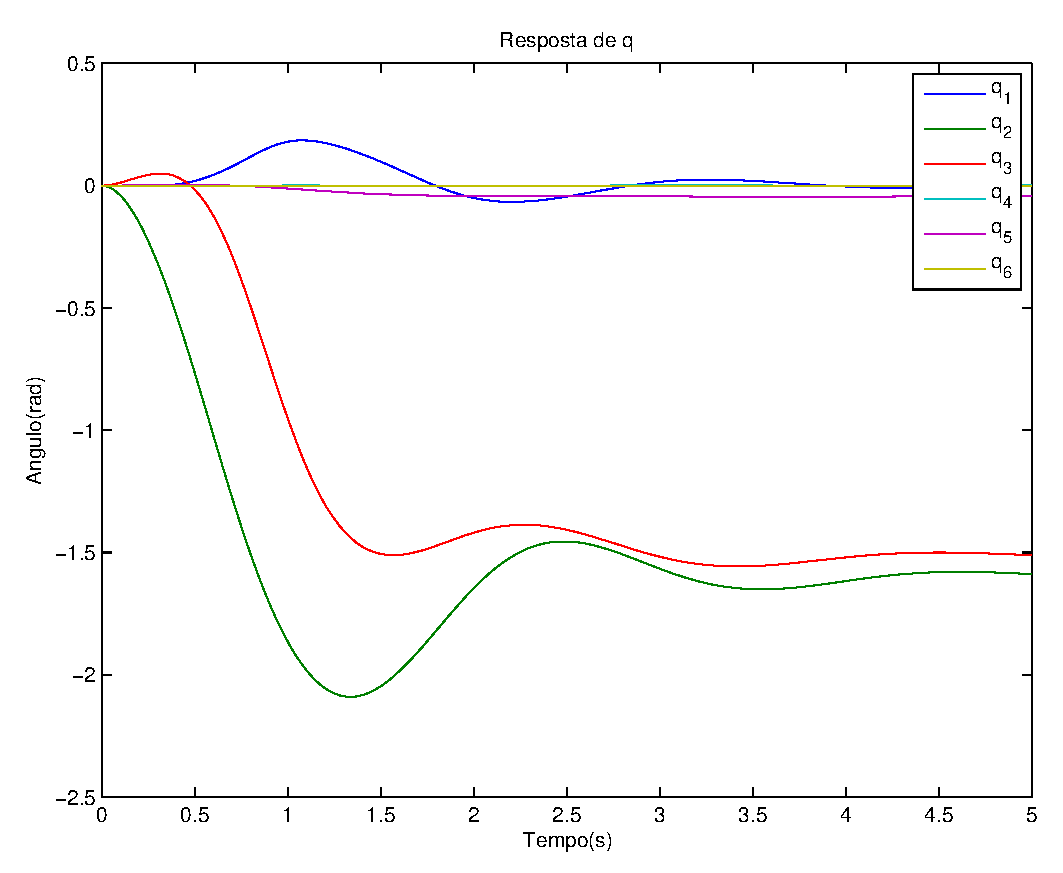
\includegraphics[width=0.8\linewidth]{../sim1ode}
	\caption{Simulação 1 para o robô Puma}
	\label{fig:pumasim1}
\end{figure}

\subsubsection{Simulação 2}
Condições iniciais:
\begin{equation}
\label{eq:sim2q}
q_{init}=\begin{bmatrix}
0 & \pi & -\frac{\pi}{2} & 0 & 0 & 0
\end{bmatrix}^T
\end{equation}
\begin{equation}
\label{eq:sim2qd}
\dot{q_{init}}=\begin{bmatrix}
0 & 0 & 0 & 0 & 0 & 0
\end{bmatrix}^T
\end{equation}

\begin{figure}[H]
	\centering
	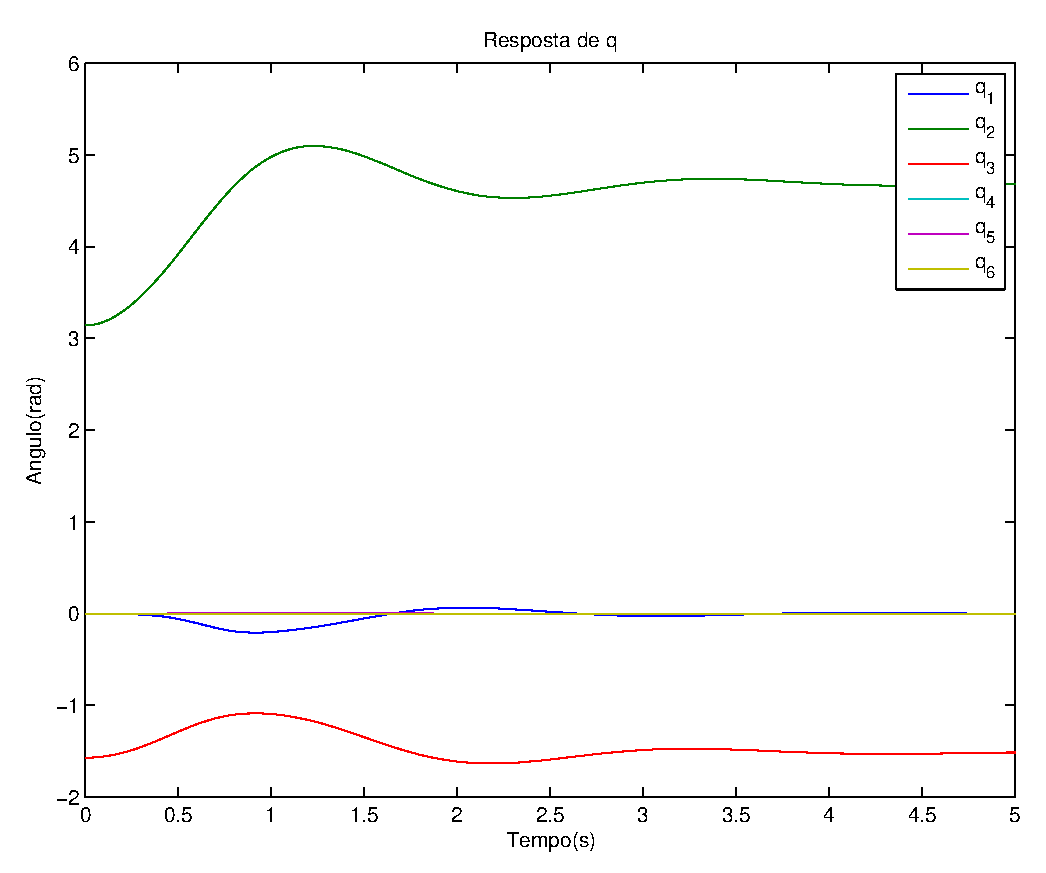
\includegraphics[width=0.8\linewidth]{../sim2ode}
	\caption{Simulação 2 para o robô Puma}
	\label{fig:pumasim2}
\end{figure}

\subsubsection{Simulação 3}
Condições iniciais:
\begin{equation}
\label{eq:sim3q}
q_{init}=\begin{bmatrix}
0 & \frac{\pi}{2} & -\frac{\pi}{2} & 0 & 0 & 0
\end{bmatrix}^T
\end{equation}
\begin{equation}
\label{eq:sim3qd}
\dot{q_{init}}=\begin{bmatrix}
0 & 0 & 0 & 0 & 0 & 0
\end{bmatrix}^T
\end{equation}

\begin{figure}[H]
	\centering
	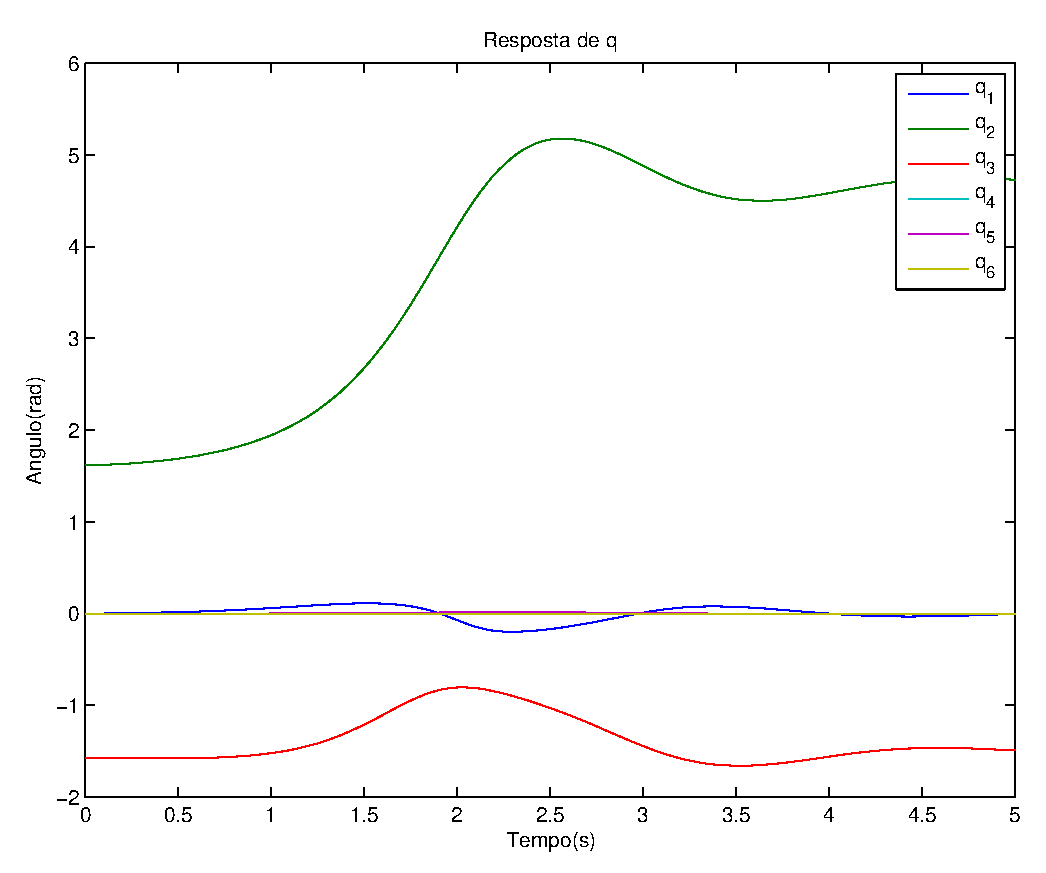
\includegraphics[width=0.8\linewidth]{../sim4ode}
	\caption{Simulação 3 para o robô Puma}
	\label{fig:pumasim3}
\end{figure}

\subsubsection{Simulação 4}
Condições iniciais:
\begin{equation}
\label{eq:sim4q}
q_{init}=\begin{bmatrix}
0 & \frac{\pi}{2}+0.05 & -\frac{\pi}{2} & 0 & 0 & 0
\end{bmatrix}^T
\end{equation}
\begin{equation}
\label{eq:sim4qd}
\dot{q_{init}}=\begin{bmatrix}
0 & 0 & 0 & 0 & 0 & 0
\end{bmatrix}^T
\end{equation}

\begin{figure}[H]
	\centering
	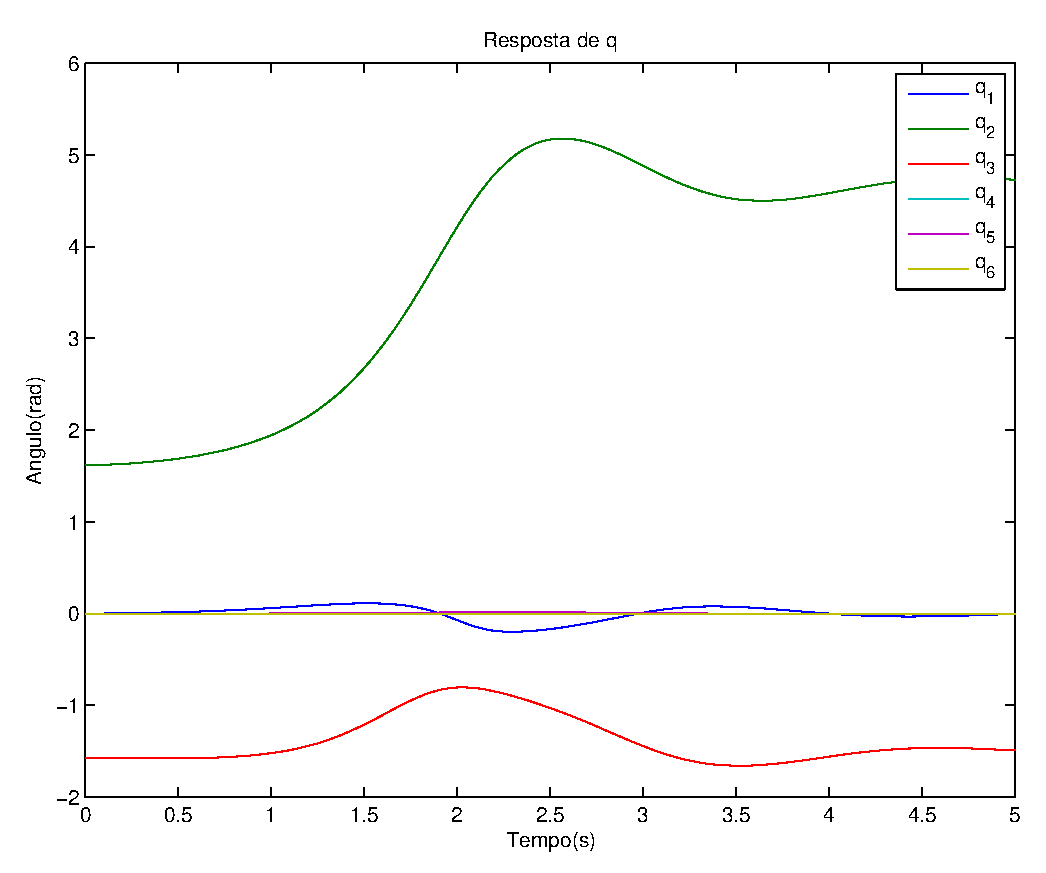
\includegraphics[width=0.8\linewidth]{../sim4ode}
	\caption{Simulação 4 para o robô Puma}
	\label{fig:pumasim4}
\end{figure}

%TODO: Comentar simulações

\subsection{Equilíbrio de energia}
A seção 6.4 da tese\cite{bb:tese} utilizada como base trata da análise de equilíbrio de energia do robô. No nosso estudo, vamos considerar nulos os esforços de compensação da força gravitacional, fazendo um estudo da energia cinética do robô Puma 560 (translação e rotação), conforme mostrado nas simulações a seguir, sendo as simulações 5 e 6 feitas com atrito viscoso (sem atrito seco), e sem atrito viscoso nem atrito seco.

\subsubsection{Simulação 5}
Condições iniciais e torque:
\begin{equation}
\label{eq:sim5q}
q_{init}=\begin{bmatrix}
0 & 0 & 0 & 0 & 0 & 0
\end{bmatrix}^T
\end{equation}
\begin{equation}
\label{eq:sim5qd}
\dot{q_{init}}=\begin{bmatrix}
0 & 0 & 0 & 0 & 0 & 0
\end{bmatrix}^T
\end{equation}
\begin{equation}
\label{eq:sim5tau}
\tau=\begin{bmatrix}
0 & 0 & 0 & 0 & 0 & 0
\end{bmatrix}^T
\end{equation}

\begin{figure}[H]
	\centering
	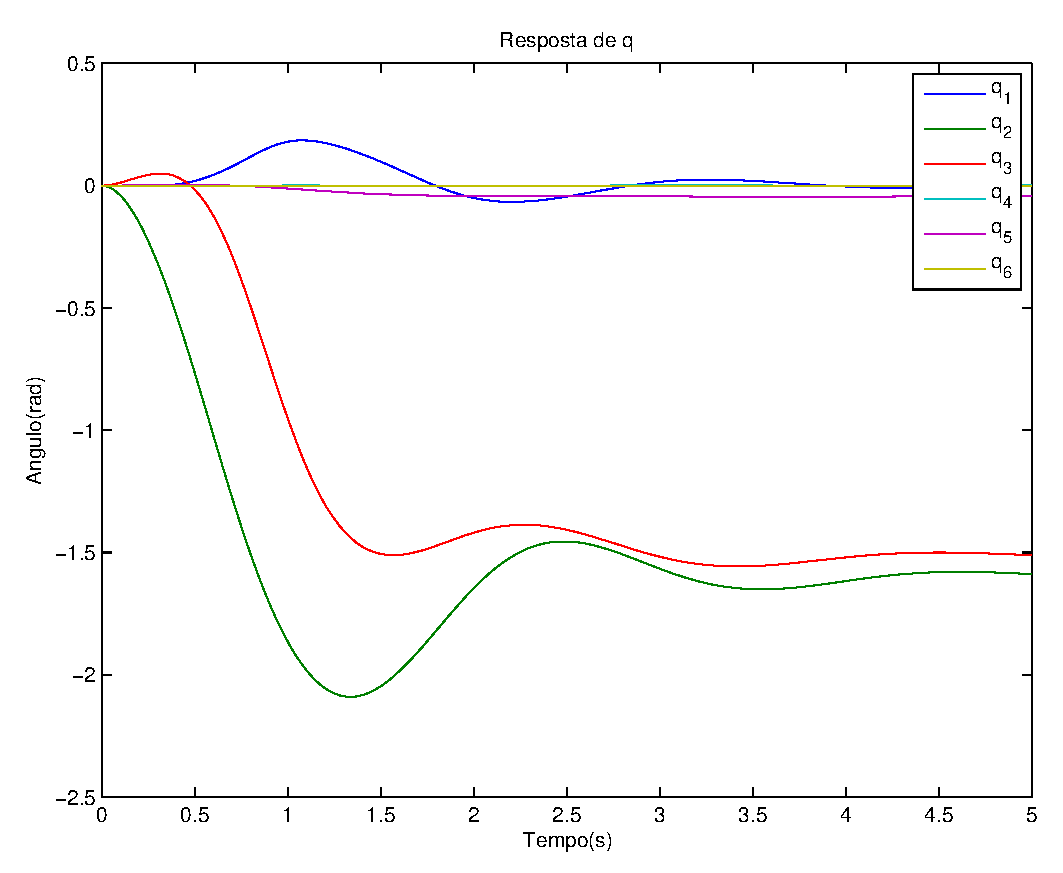
\includegraphics[width=0.8\linewidth]{../sime1odea}
	\caption{Simulação 5 para o robô Puma com atrito viscoso}
	\label{fig:pumasim5}
\end{figure}

\begin{figure}[H]
	\centering
	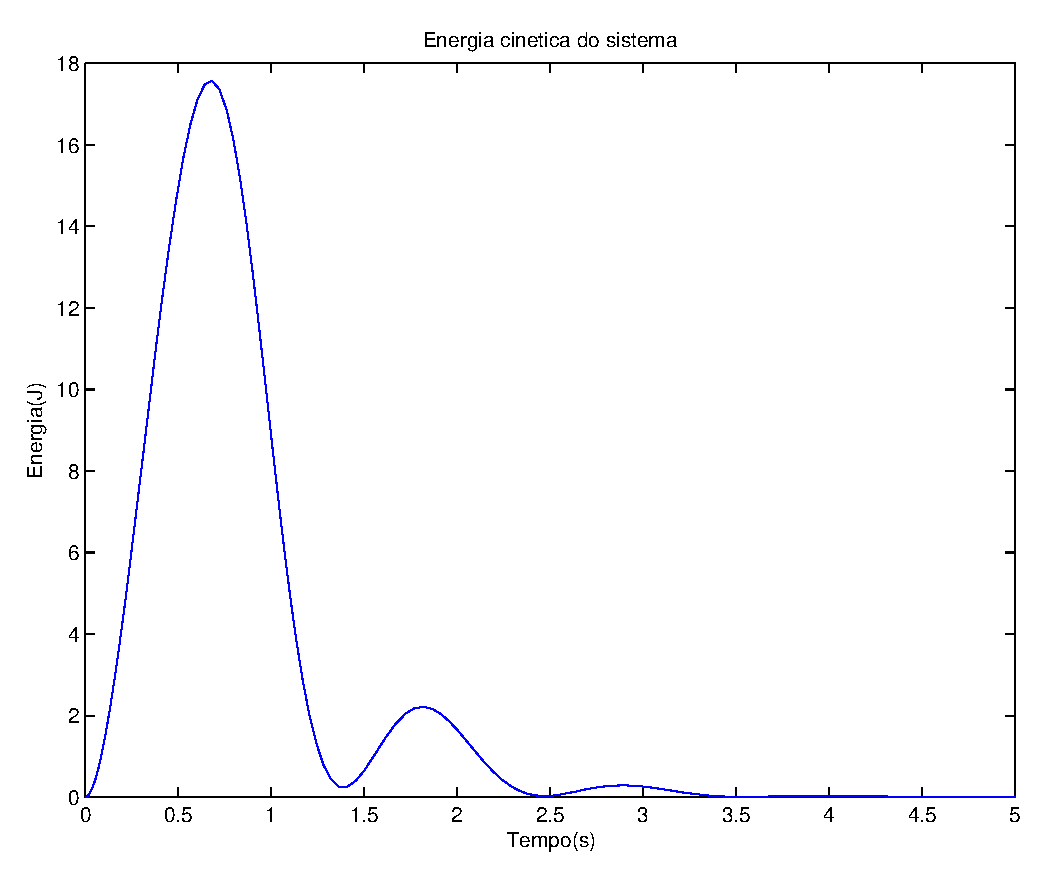
\includegraphics[width=0.8\linewidth]{../sime1kina}
	\caption{Simulação 5 para energia do robô Puma com atrito viscoso}
	\label{fig:energysim5}
\end{figure}

\begin{figure}[H]
	\centering
	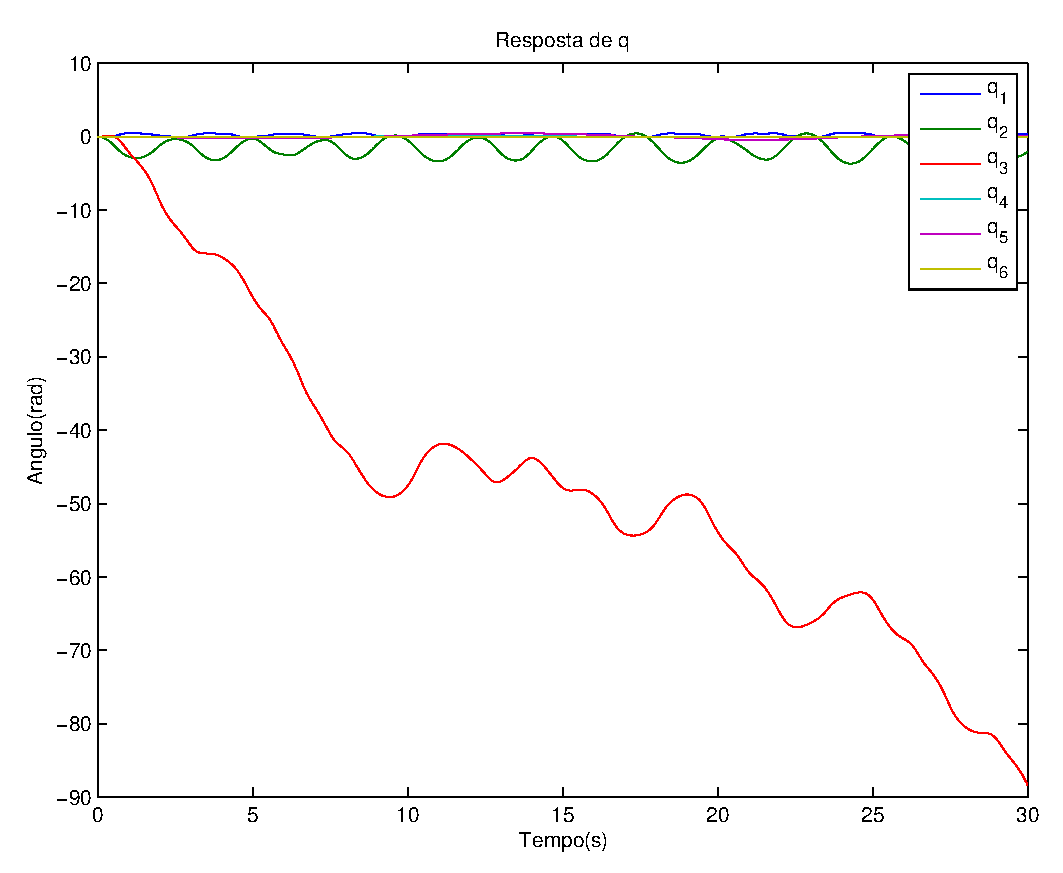
\includegraphics[width=0.8\linewidth]{../longsims/sime1ode.eps}
	\caption{Simulação 5 para o robô Puma sem atrito viscoso}
	\label{fig:pumasim5nf}
\end{figure}

\begin{figure}[H]
	\centering
	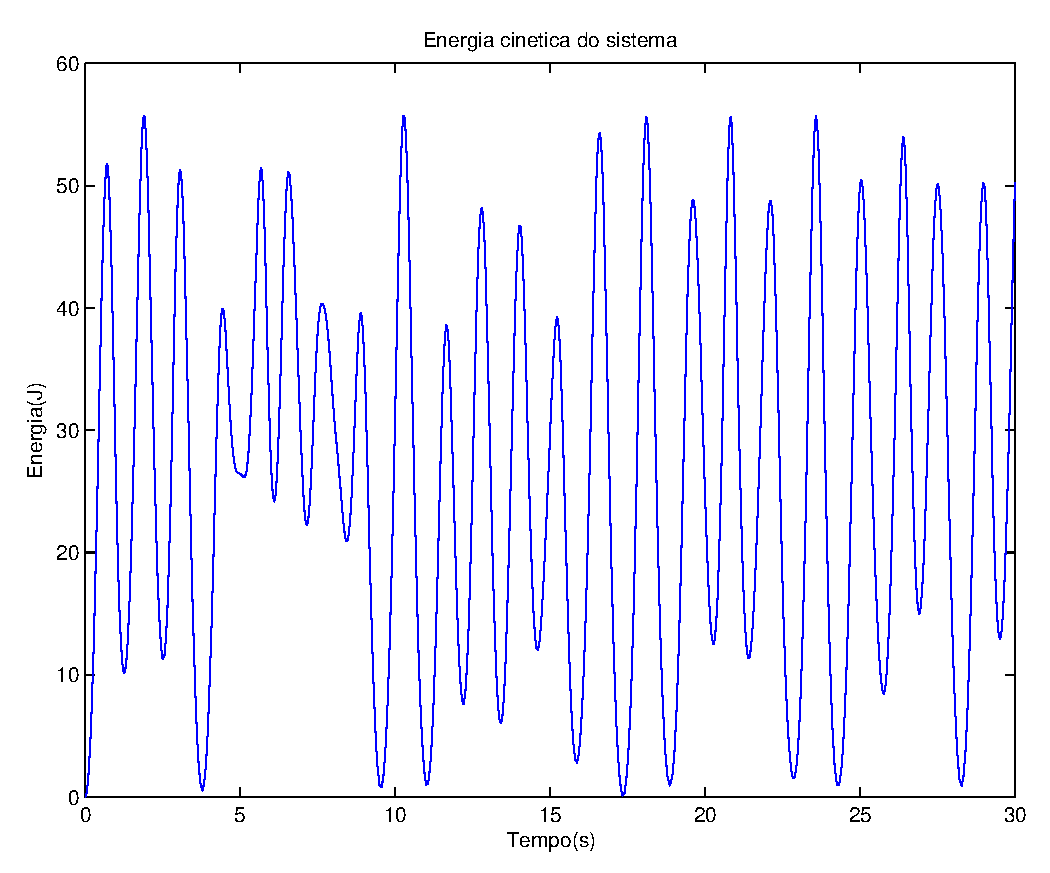
\includegraphics[width=0.8\linewidth]{../longsims/sime1kin.eps}
	\caption{Simulação 5 para energia do robô Puma sem atrito viscoso}
	\label{fig:energysim5nf}
\end{figure}

\subsubsection{Simulação 6}
Condições iniciais e torque:
\begin{equation}
\label{eq:sim6q}
q_{init}=\begin{bmatrix}
0 & 0.000001 & 0 & 0 & 0 & 0
\end{bmatrix}^T
\end{equation}
\begin{equation}
\label{eq:sim6qd}
\dot{q_{init}}=\begin{bmatrix}
0 & 0 & 0 & 0 & 0 & 0
\end{bmatrix}^T
\end{equation}
\begin{equation}
\label{eq:sim6tau}
\tau=\begin{bmatrix}
0 & 0 & 0 & 0 & 0 & 0
\end{bmatrix}^T
\end{equation}

\begin{figure}[H]
	\centering
	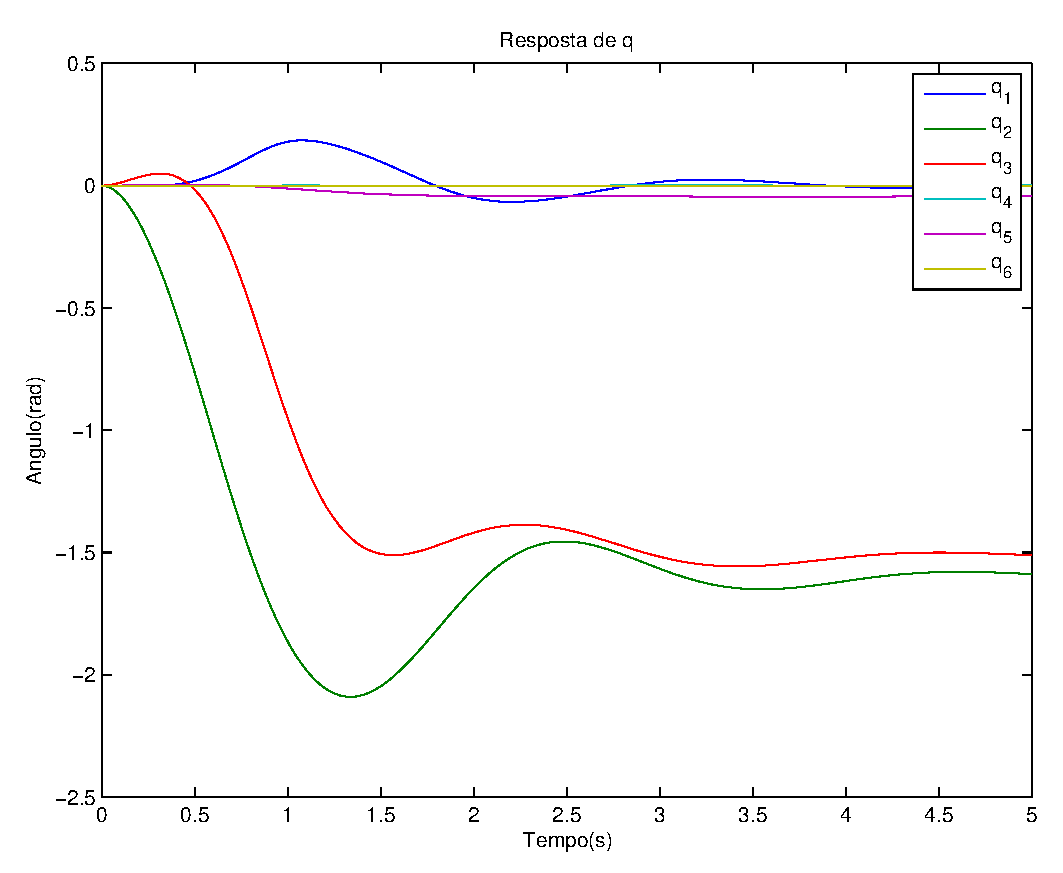
\includegraphics[width=0.8\linewidth]{../sime2odea}
	\caption{Simulação 6 para o robô Puma com atrito viscoso}
	\label{fig:pumasim6}
\end{figure}

\begin{figure}[H]
	\centering
	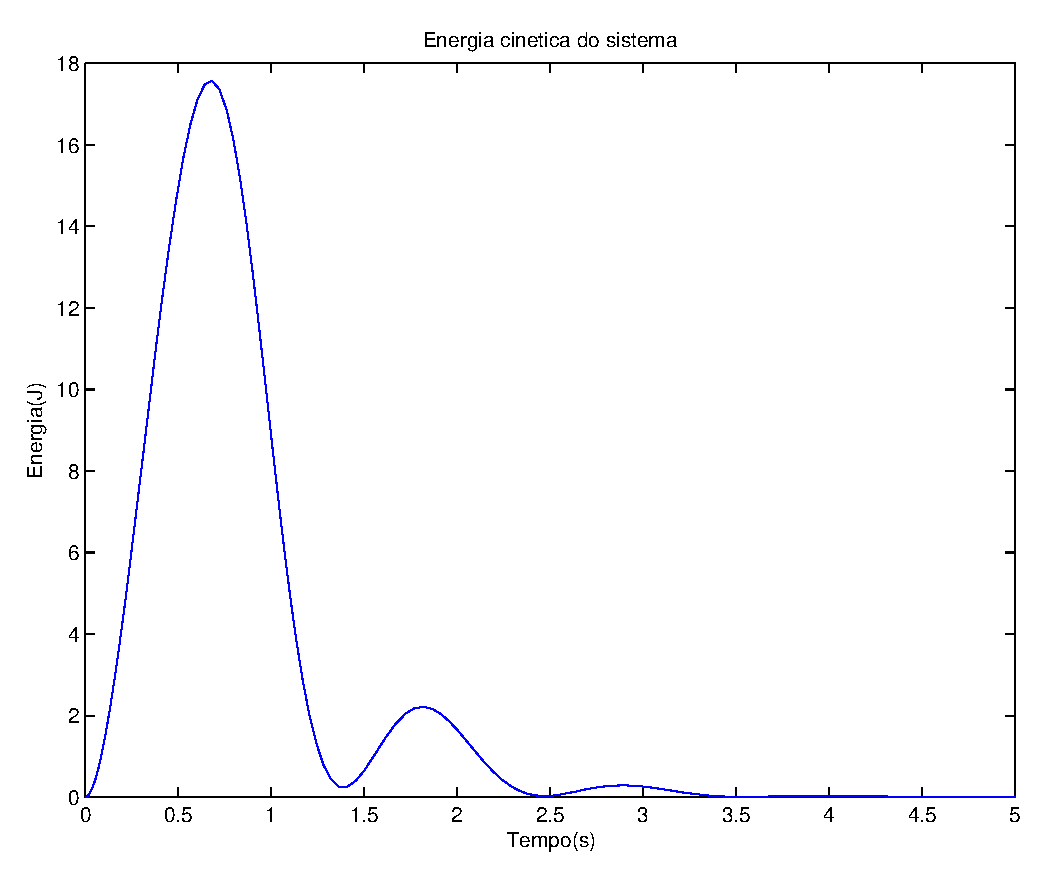
\includegraphics[width=0.8\linewidth]{../sime1kina}
	\caption{Simulação 6 para energia o robô Puma com atrito viscoso}
	\label{fig:energysim6}
\end{figure}

\begin{figure}[H]
	\centering
	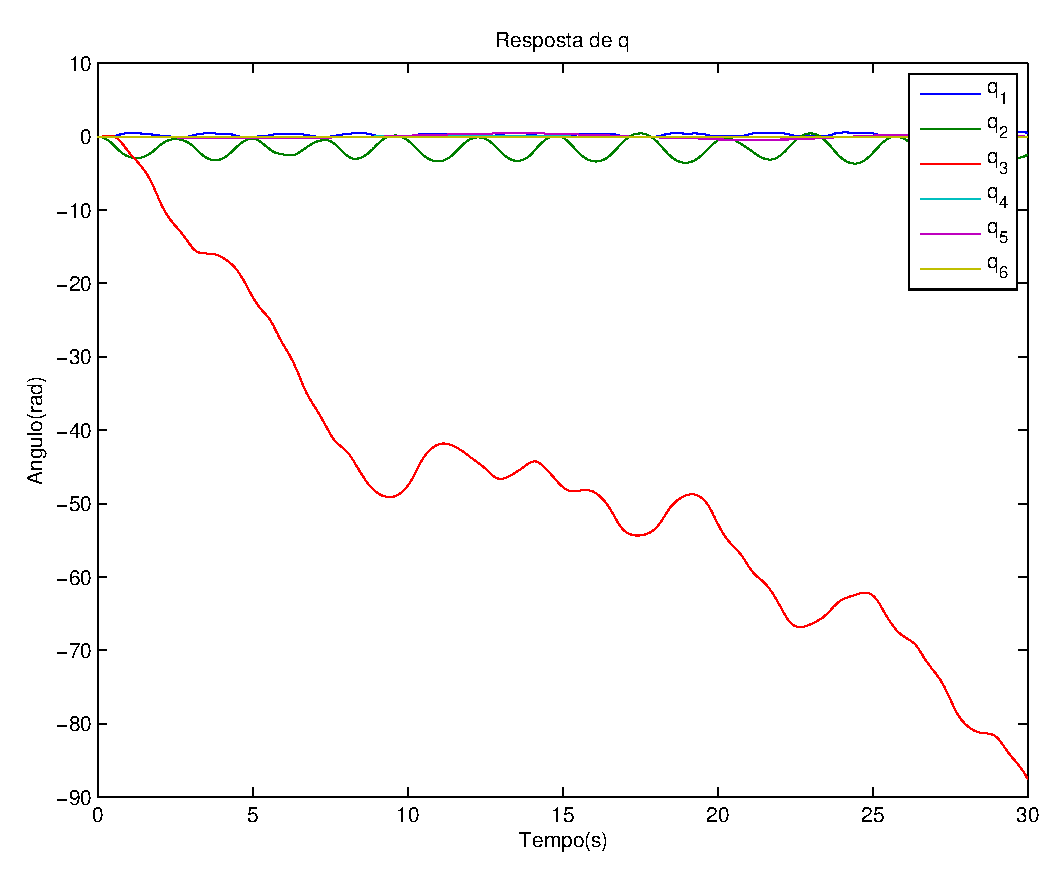
\includegraphics[width=0.8\linewidth]{../longsims/sime2ode.eps}
	\caption{Simulação 6 para o robô Puma sem atrito viscoso}
	\label{fig:pumasim6nf}
\end{figure}

\begin{figure}[H]
	\centering
	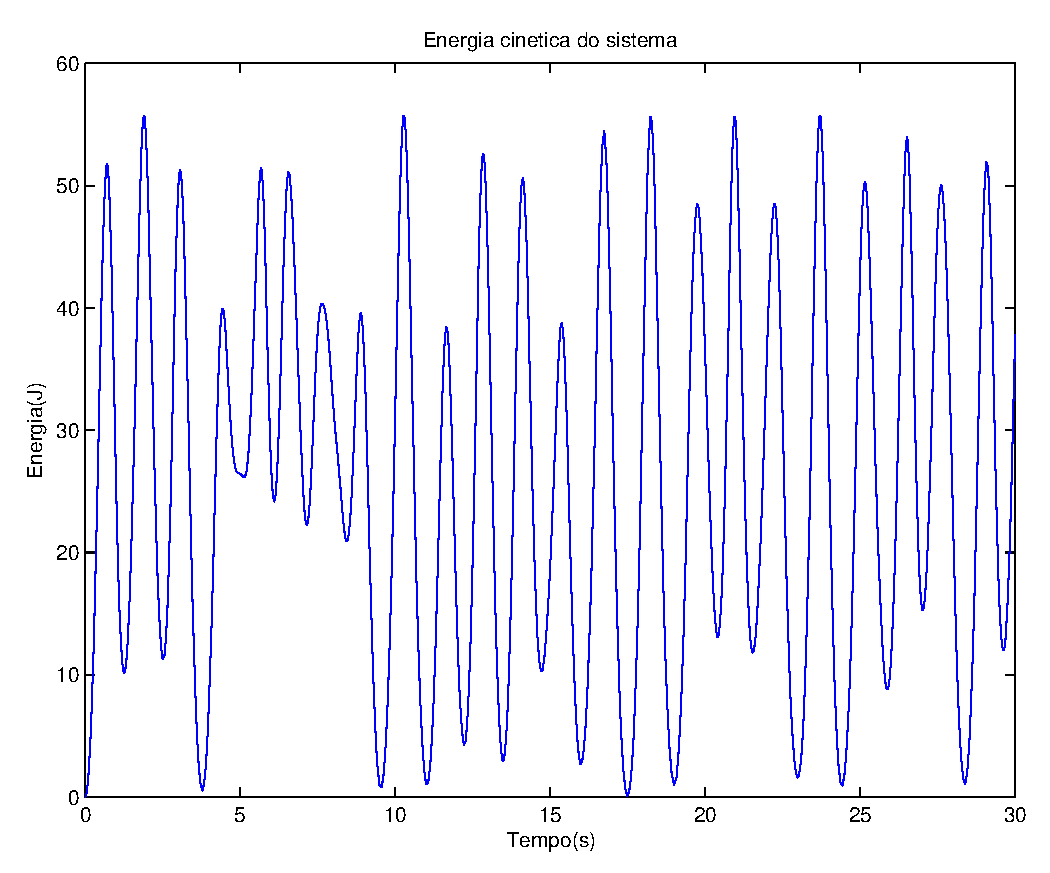
\includegraphics[width=0.8\linewidth]{../longsims/sime2kin.eps}
	\caption{Simulação 6 para energia do robô Puma sem atrito viscoso}
	\label{fig:energysim6nf}
\end{figure}

%TODO: Comentar simulações

\subsection{Controle em malha fechada}



\section{Cinemática}
\subsection{Controle de Trajetória}
\subsection{Elipse}

\section{Questões}
\begin{itemize}
	\item \textbf{Por que na seção ``Controle em malha fechada" os torques finais obtidos são nulos? O torque final não deveria ser igual ao torque de compensação da força da gravidade?}
	
	\item \textbf{Na seção ``Equilíbrio de energia cinética" foi indicado um comando do Matlab para se obter a matriz de massa/inércia no espaço das juntas $\rightarrow M(q)$. Como você faria para obter essa matriz de massa utilizando o método de Newton-Euler além de manipulação simbólica? Veja os apêndices B e C da tese\cite{bb:tese}. Essa matriz corresponde à matriz $M(q)$ da equação geral da dinâmica de um robô, como dado abaixo, onde ``u" é o vetor de torques nas juntas.}
	
	\begin{equation}
	\label{eq:mq}
	M(q)\ddot{q}+C(q,\dot{q})\dot{q}+g(q)=u
	\end{equation}
	
	\item \textbf{Por que essa matriz de massa $M(q)$ não é do tipo da matriz de massa abaixo de um corpo rígido, que é uma matriz $6x6$ com uma matriz diagonal $M$ e outra matriz de inércia do corpo J?}
	
	\begin{equation}
	\label{eq:m6x6}
	\bar{M}=\begin{bmatrix}
	M & 0\\
	0 & J
	\end{bmatrix}
	\end{equation}
	
	
\end{itemize}

\begin{thebibliography}{widestlabel}
	\bibitem{bb:roteiro}{Roteiro do projeto disponibilizado para os alunos}
	\bibitem{bb:toolbox}{Peter Corke, Robotics Toolbox, disponível em http://www.petercorke.com/Robotics\_Toolbox.html}
	\bibitem{bb:inirbt}{Código ini\_Rbt.m fornecido pelo professor}
	\bibitem{bb:rbtsquare}{Código Rbtsquare.m fornecido pelo professor}
	\bibitem{bb:tese}{Herman Høifødt, Dynamic Modeling and Simulation of Robot Manipulators, The Newton-Euler Formulation, disponível em http://www.diva-portal.org/smash/get/diva2:436733/FULLTEXT01.pdf}
	
\end{thebibliography}
\end{document}

